\documentclass{article}
\usepackage{enumitem}
\usepackage{listings}
\usepackage{xcolor}
\usepackage{graphicx}
\usepackage{pxfonts}
\graphicspath{ {./Immagini/} }

\definecolor{backcolour}{rgb}{0.98,0.98,0.98}
\definecolor{darkmagenta}{rgb}{0.55, 0.0, 0.55}
\definecolor{forestgreen(web)}{rgb}{0.13, 0.55, 0.13}
\definecolor{codegray}{rgb}{0.5,0.5,0.5}
\definecolor{chromeyellow}{rgb}{1.0, 0.65, 0.0}

\lstdefinestyle{mystyle}{
    backgroundcolor=\color{backcolour},
    commentstyle=\color{darkmagenta} \textit,
    keywordstyle=\color{forestgreen(web)} \textbf,
    numberstyle=\tiny\color{codegray},
    stringstyle=\color{chromeyellow},
    basicstyle=\ttfamily\footnotesize,
    breakatwhitespace=false,
    breaklines=true,
    captionpos=b,
    keepspaces=true,
    numbers=left,
    numbersep=5pt,
    showspaces=false,
    showstringspaces=false,
    showtabs=false,
    tabsize=2
}

\lstdefinestyle{myPythonStyle}{
    backgroundcolor=\color{white},
}

\lstset{style=mystyle}

\title{Genome sequence research}
\author{\\Carmelo Santamaria (514926) \\ Federico Sciuto (517075)}
\date{Novembre 2023}

\begin{document}
    
    \maketitle
    
    \vspace{10pt}
    
    \section{Introduzione}
    Il genoma è l’insieme del patrimonio genetico che caratterizza ogni organismo vivente.
    Il genoma umano è costituito da 25 differenti molecole di DNA. Poiché la quantità di DNA nucleare è preponderante rispetto a quello mitocondriale, per genoma si intende spesso l’insieme delle molecole di DNA cromosomico, più correttamente chiamato genoma nucleare. Nell'uomo il genoma nucleare è costituito da circa 3.200 Mb (Mb = megabasi, o milioni di paia di basi), comprendenti circa 25.000 geni, localizzati sui cromosomi. Il genoma mitocondriale consiste di un DNA circolare a doppio filamento lungo 16,6 kb e contenente 37 geni, presente in molte copie nei mitocondri. Qualsiasi cellula di un organismo umano possiede lo stesso genoma (genoma equivalente): infatti è l’espressione differenziale dei geni, alla base dello sviluppo embrionale, che rende diversi i vari tipi cellulari.
    
    \vspace{20pt}
    
    \section{Frameworks}
    
    \subsection{MapReduce}
    MapReduce è un modello di programmazione che viene eseguito su Hadoop, un motore di analisi dati ampiamente utilizzato per i Big Data e scrive applicazioni che vengono eseguite in parallelo per elaborare grandi volumi di dati archiviati su cluster.
    
    Il funzionamento di MapReduce può essere suddiviso in tre fasi, di cui 2 principali (Map e Reduce), con una quarta fase facoltativa (Combiner).
    
    \begin{itemize}
        \item
        \textbf{Mapper:} in questa prima fase, la logica condizionale filtra i dati attraverso tutti i nodi in coppie chiave-valore. La "chiave" si riferisce all'indirizzo di offset per ogni record, mentre il "valore" contiene l’intero contenuto del record.
        
        \item
        \textbf{Shuffle:} durante la seconda fase, i valori di output dalla mappatura vengono ordinati e consolidati. I valori vengono raggruppati in base a chiavi simili e i quelli duplicati vengono scartati. Anche l’output della fase Shuffle è organizzato in coppie chiave-valore, ma questa volta i valori indicano un intervallo e non il contenuto di un record.
        
        \item
        \textbf{Reducer:} nella terza fase, l'output della fase Shuffle consolidato viene aggregato, con tutti i valori aggiunti alle chiavi corrispondenti. Tutto questo viene quindi combinato in una singola directory di output.
        
        \item
        \textbf{Combiner:} l'esecuzione di questa fase può ottimizzare le prestazioni dei processi MapReduce, accelerandone il flusso. Per effettuare questa operazione MapReduce recupera gli output della fase Mapper e li esamina a livello di nodo per individuare duplicati, che vengono combinati in una singola coppia chiave-valore, riducendo in questo modo il processo che la fase Shuffle deve completare.
    \end{itemize}
    
    \begin{figure}[h!]
        \centering
        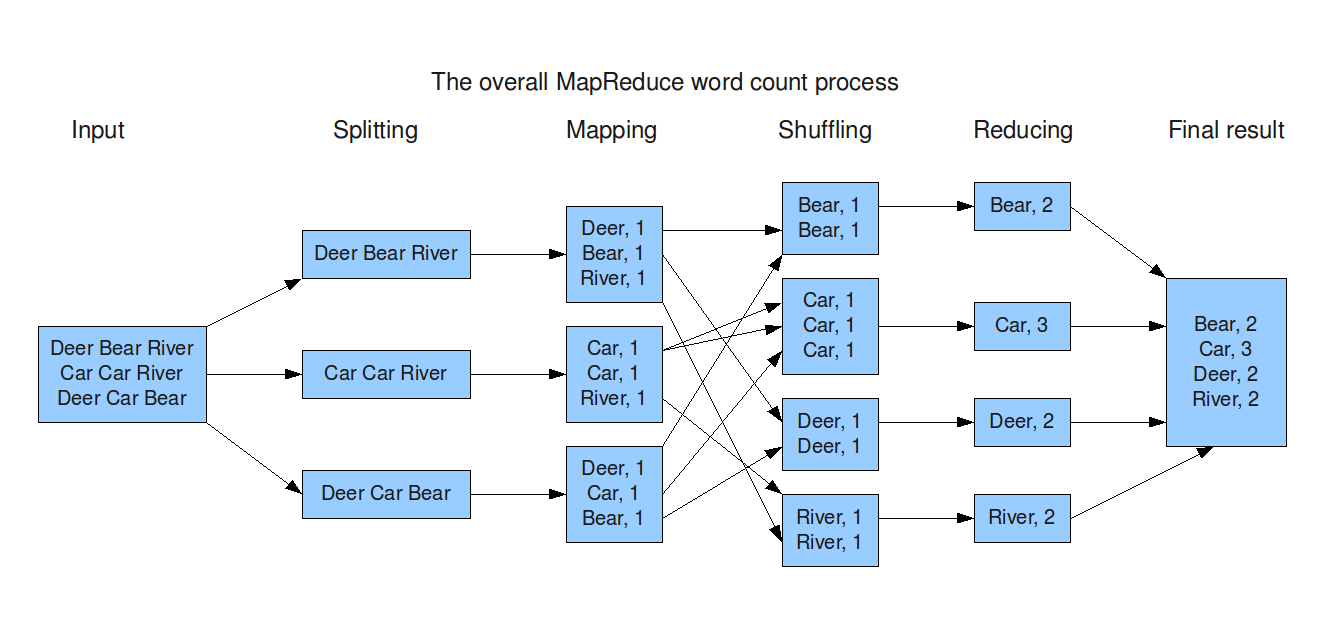
\includegraphics[width=\linewidth]{Schema MapReduce.png}
        \caption{Schema di esempio del MapReduce}
    \end{figure}
    
    \clearpage
    \subsection{Ray}
    Ray è un framework open source versatile che offre una piattaforma unificata per la gestione e l'elaborazione di carichi di lavoro AI e Python su larga scala, con l'obiettivo principale di semplificare il processo di sviluppo e distribuzione di applicazioni di intelligenza artificiale. Fornisce agli sviluppatori gli strumenti necessari per sfruttare al meglio le risorse del sistema.\\
    \\
    Il cuore di Ray è costituito dai cluster Ray, che consentono di distribuire e gestire in modo efficiente i carichi di lavoro. Un cluster Ray è composto da: un nodo principale (head) responsabile della coordinazione generale e dell'allocazione delle risorse, e un insieme di nodi di lavoro (worker) che eseguono i task specifici.\\
    \\
    Gli sviluppatori possono definire i loro carichi di lavoro come task paralleli o processi, che vengono quindi distribuiti tra i nodi di lavoro all'interno del cluster Ray. Questo modello parallelo consente di sfruttare al meglio le risorse disponibili, accelerando notevolmente l'elaborazione di compiti intensivi, come l'addestramento di modelli di machine learning o la simulazione nell'apprendimento per rinforzo.
    
    \vspace{10pt}
    
    \begin{figure}[h!]
        \centering
        \includegraphics[width=\linewidth]{Architettura Ray cluster.jpg}
        \caption{Schema di esempio del funzionamento di un cluster Ray}
    \end{figure}
    
    \clearpage
    
    \section{Codice}
    Il codice è stato scritto in Python, un linguaggio di programmazione noto per la sua semplicità e vantaggioso per la sua ampia libreria standard. L'ambiente di sviluppo in cui il codice è stato creato e testato è Ubuntu 22.04 LTS, un sistema operativo stabile e leggero, che offre un ottimo supporto per Python e la libreria Ray.
    Per l'implementazione di alcune funzionalità specifiche, sono state utilizzate le seguenti librerie e moduli:

    \vspace{5pt}
    
    \begin{lstlisting}[language=Python, style=myPythonStyle]
from Bio import SeqIO                                                  # Modulo della libreria Biopython, utilizzato per lavorare con sequenze biologiche (sequenze di DNA, RNA e proteine). SeqIO permette la lettura e la scrittura di file contenenti queste sequenze
from time import perf_counter                                          # Funzione del modulo time che restituisce un tempo di clock per misurare il tempo trascorso tra due punti in un programma
from functools import reduce                                           # Funzione del modulo functools che consente di applicare una funzione cumulativa a elementi di un iterabile, riducendo la sequenza a un singolo valore. Usato per eseguire operazioni di aggregazione su una sequenza di dati.
import multiprocessing                                                 # Libreria che fornisce supporto per la programmazione concorrente, consentendo di eseguire processi multipli contemporaneamente per sfruttare i multi-core delle CPU
from multiprocessing import cpu_count                                  # Funzione che restituisce il numero di core della CPU disponibili sul sistema in uso
import ray                                                             # Libreria per la programmazione parallela e distribuita in Python
\end{lstlisting}

    \vspace{5pt}
    
    Per i test del codice multithread è stata utilizzata una macchina con 12 thread, che è stata il nodo "head" nel cluster utilizzato con la versione Ray, affiancato da altri 9 nodi "worker" con 4 thread ciascuno; per un totale di 10 nodi e 48 thread.

    \vspace{5pt}
    
    \subsection{Monothread}
    Nel codice Monothread il lavoro è stato suddiviso tra le funzioni:
    
    \begin{enumerate}
        \item \textbf{"Mapping"}, la funzione di mappatura, che
        \begin{itemize}
            \item Prende in ingresso:
            \begin{itemize}
                \item sequenza (una sequenza genetica);
                \item stringa\_target (la stringa da cercare in sequenza);
            \end{itemize}
            \item Calcola la "\textit{lunghezza\_target}", cioè la lunghezza della "\textit{stringa\_target}".
            \item Crea una lista di sottosequenze attraverso una list comprehension contenente tutte le sottosequenze di sequenza che hanno la stessa lunghezza di "\textit{stringa\_target}".
            \item Restituisce la lista "\textit{sottosequenze}".
        \end{itemize}

        \item \textbf{“Reducing”}, la funzione di riduzione, che
        \begin{itemize}
            \item Prende in ingresso:
            \begin{itemize}
                \item sottosequenze (la lista di sottosequenze create dalla funzione \textit{mapping});
                \item stringa\_target;
            \end{itemize}
            \item Calcola il "\textit{conteggio}", ovvero quante volte "\textit{stringa\_target}" appare in "\textit{sottosequenze}" utilizzando il 
metodo \textbf{\textit{count()}}.
            \item Restituisce il "\textit{conteggio}".
        \end{itemize}

        \item \textbf{"Conteggio\_finale"}, che
        \begin{itemize}
            \item Prende in ingresso i conteggi intermedi:
            \begin{itemize}
                \item count1;
                \item count2;
            \end{itemize}
            \item Restituisce la loro somma.
        \end{itemize}

        \item \textbf{"MapReduce"}, la funzione principale che esegue l'analisi MapReduce attraverso le funzioni definite precedentemente.
        \\Essa:
        \begin{itemize}
            \item Registra il tempo di inizio dell'esecuzione
            \item Utilizza \textbf{\textit{map()}} per applicare la funzione \textbf{\textit{lambda}} a ciascuna sequenza in "\textit{data}". La funzione \textbf{\textit{lambda}} prende una sequenza, esegue la funzione \textbf{\textit{reducing}} sulla sequenza utilizzando la "\textit{stringa\_target}" e restituisce il "\textit{conteggio}".
            \item Utilizza \textbf{\textit{reduce()}} per sommare i conteggi intermedi e calcolare il "\textit{conteggio\_totale}".
            \item Registra il tempo di fine esecuzione.
            \item Stampa il risultato, indicando quante volte la "\textit{stringa\_target}" è presente nel file e quanto tempo è stato necessario per l'analisi.
        \end{itemize}
    \end{enumerate}

    
    \vspace{10pt}
    
    \lstinputlisting[language=Python]{Codici/RicercaStringa_Mono.py}

    \clearpage
    
    \subsection{Multithread}
    L'implementazione del codice Multithread è molto simile a quella vista nel Monothread, con la differenza che vengono utilizzati la libreria \textbf{\textit{"Multiprocessing"}} e il modulo \textbf{\textit{"cpu\_count"}} per supportare il parallelismo; è stata, inoltre, modificata la funzione \textbf{\textit{"MapReduce"}} e inserita una nuova funzione:

    \begin{enumerate}
        \item \textbf{"Process\_chunk"}, definita per suddividere il lavoro fra i vari core, che
        \begin{itemize}
            \item Prende in ingresso:
            \begin{itemize}
                \item chunk di dati (un sottoinsieme delle sequenze genetiche);
                \item stringa\_target;
            \end{itemize}
        \item Esegue la fase di \textbf{\textit{mapping}} e \textbf{\textit{reducing}} sulle sequenze all'interno del "\textit{chunk}"
        \item Restituisce il "\textit{conteggio}"
        \end{itemize}
    \end{enumerate}
    \\Le modifiche nella funzione \textbf{"MapReduce"} consistono in:
    \begin{itemize}
        \item Una divisione dei dati in "\textit{chunk}" per la parallelizzazione, calcolando il "\textit{chunk\_size}" in base al numero di processi specificato.
        \item Uso di un pool di processi (\textit{multiprocessing.Pool}) per distribuire il lavoro sui "\textit{chunk}" ai processi paralleli utilizzando "\textit{pool.starmap}".
        \item La somma dei conteggi intermedi prodotti dai processi paralleli per ottenere il "\textit{conteggio totale}".
        \item La possibilità di scegliere il numero di processi da utilizzare per il parallelismo utilizzando "\textit{multiprocessing.cpu\_count()}" per ottenere il numero massimo di core disponibili sulla macchina.
    \end{itemize}
    
    \vspace{10pt}
    
    \lstinputlisting[language=Python]{Codici/RicercaStringa_Multi.py}

    \vspace{5pt}
    
    \subsection{Ray}
    Anche nel codice Ray l'implementazione è molto simile a quelle viste in precedenza; le differenze, oltre all'utilizzo della libreria \textbf{\textit{"ray"}}, sono:

    \begin{itemize}
        \item L'esecuzione della libreria \textbf{\textit{"ray.init()"}} per inizializzare il framework \textbf{Ray}.
        \item L'annotazione della funzione \textbf{\textit{process\_chunk}} con \textbf{\textit{"@ray.remote"}}, che permette a questa funzione di essere eseguita in modo parallelo da \textbf{Ray}.
        \item Anche in questo caso, così come per il Multithreading si ha la possibilità di scegliere il numero di processi da utilizzare, ma per ottenere il numero massimo di core disponibili sul cluster stavolta sono stati utilizzati:
        \begin{itemize}
            \item cluster\_resources = ray.cluster\_resources()
            \item num\_process\_max = int(cluster\_resources.get("CPU", 1))
        \end{itemize}
    \end{itemize}
    
    \vspace{10pt}
    
    \lstinputlisting[language=Python]{Codici/RicercaStringa_Ray.py}
    
    \clearpage
    
    \section{Risultati}
    Di seguito sono riportate le medie dei tempi d'esecuzione delle prove effettuate. Rappresentate sia con un grafico, che con una tabella.
    
    \vspace{10pt}
    
    \begin{figure}[h!]
        \centering
        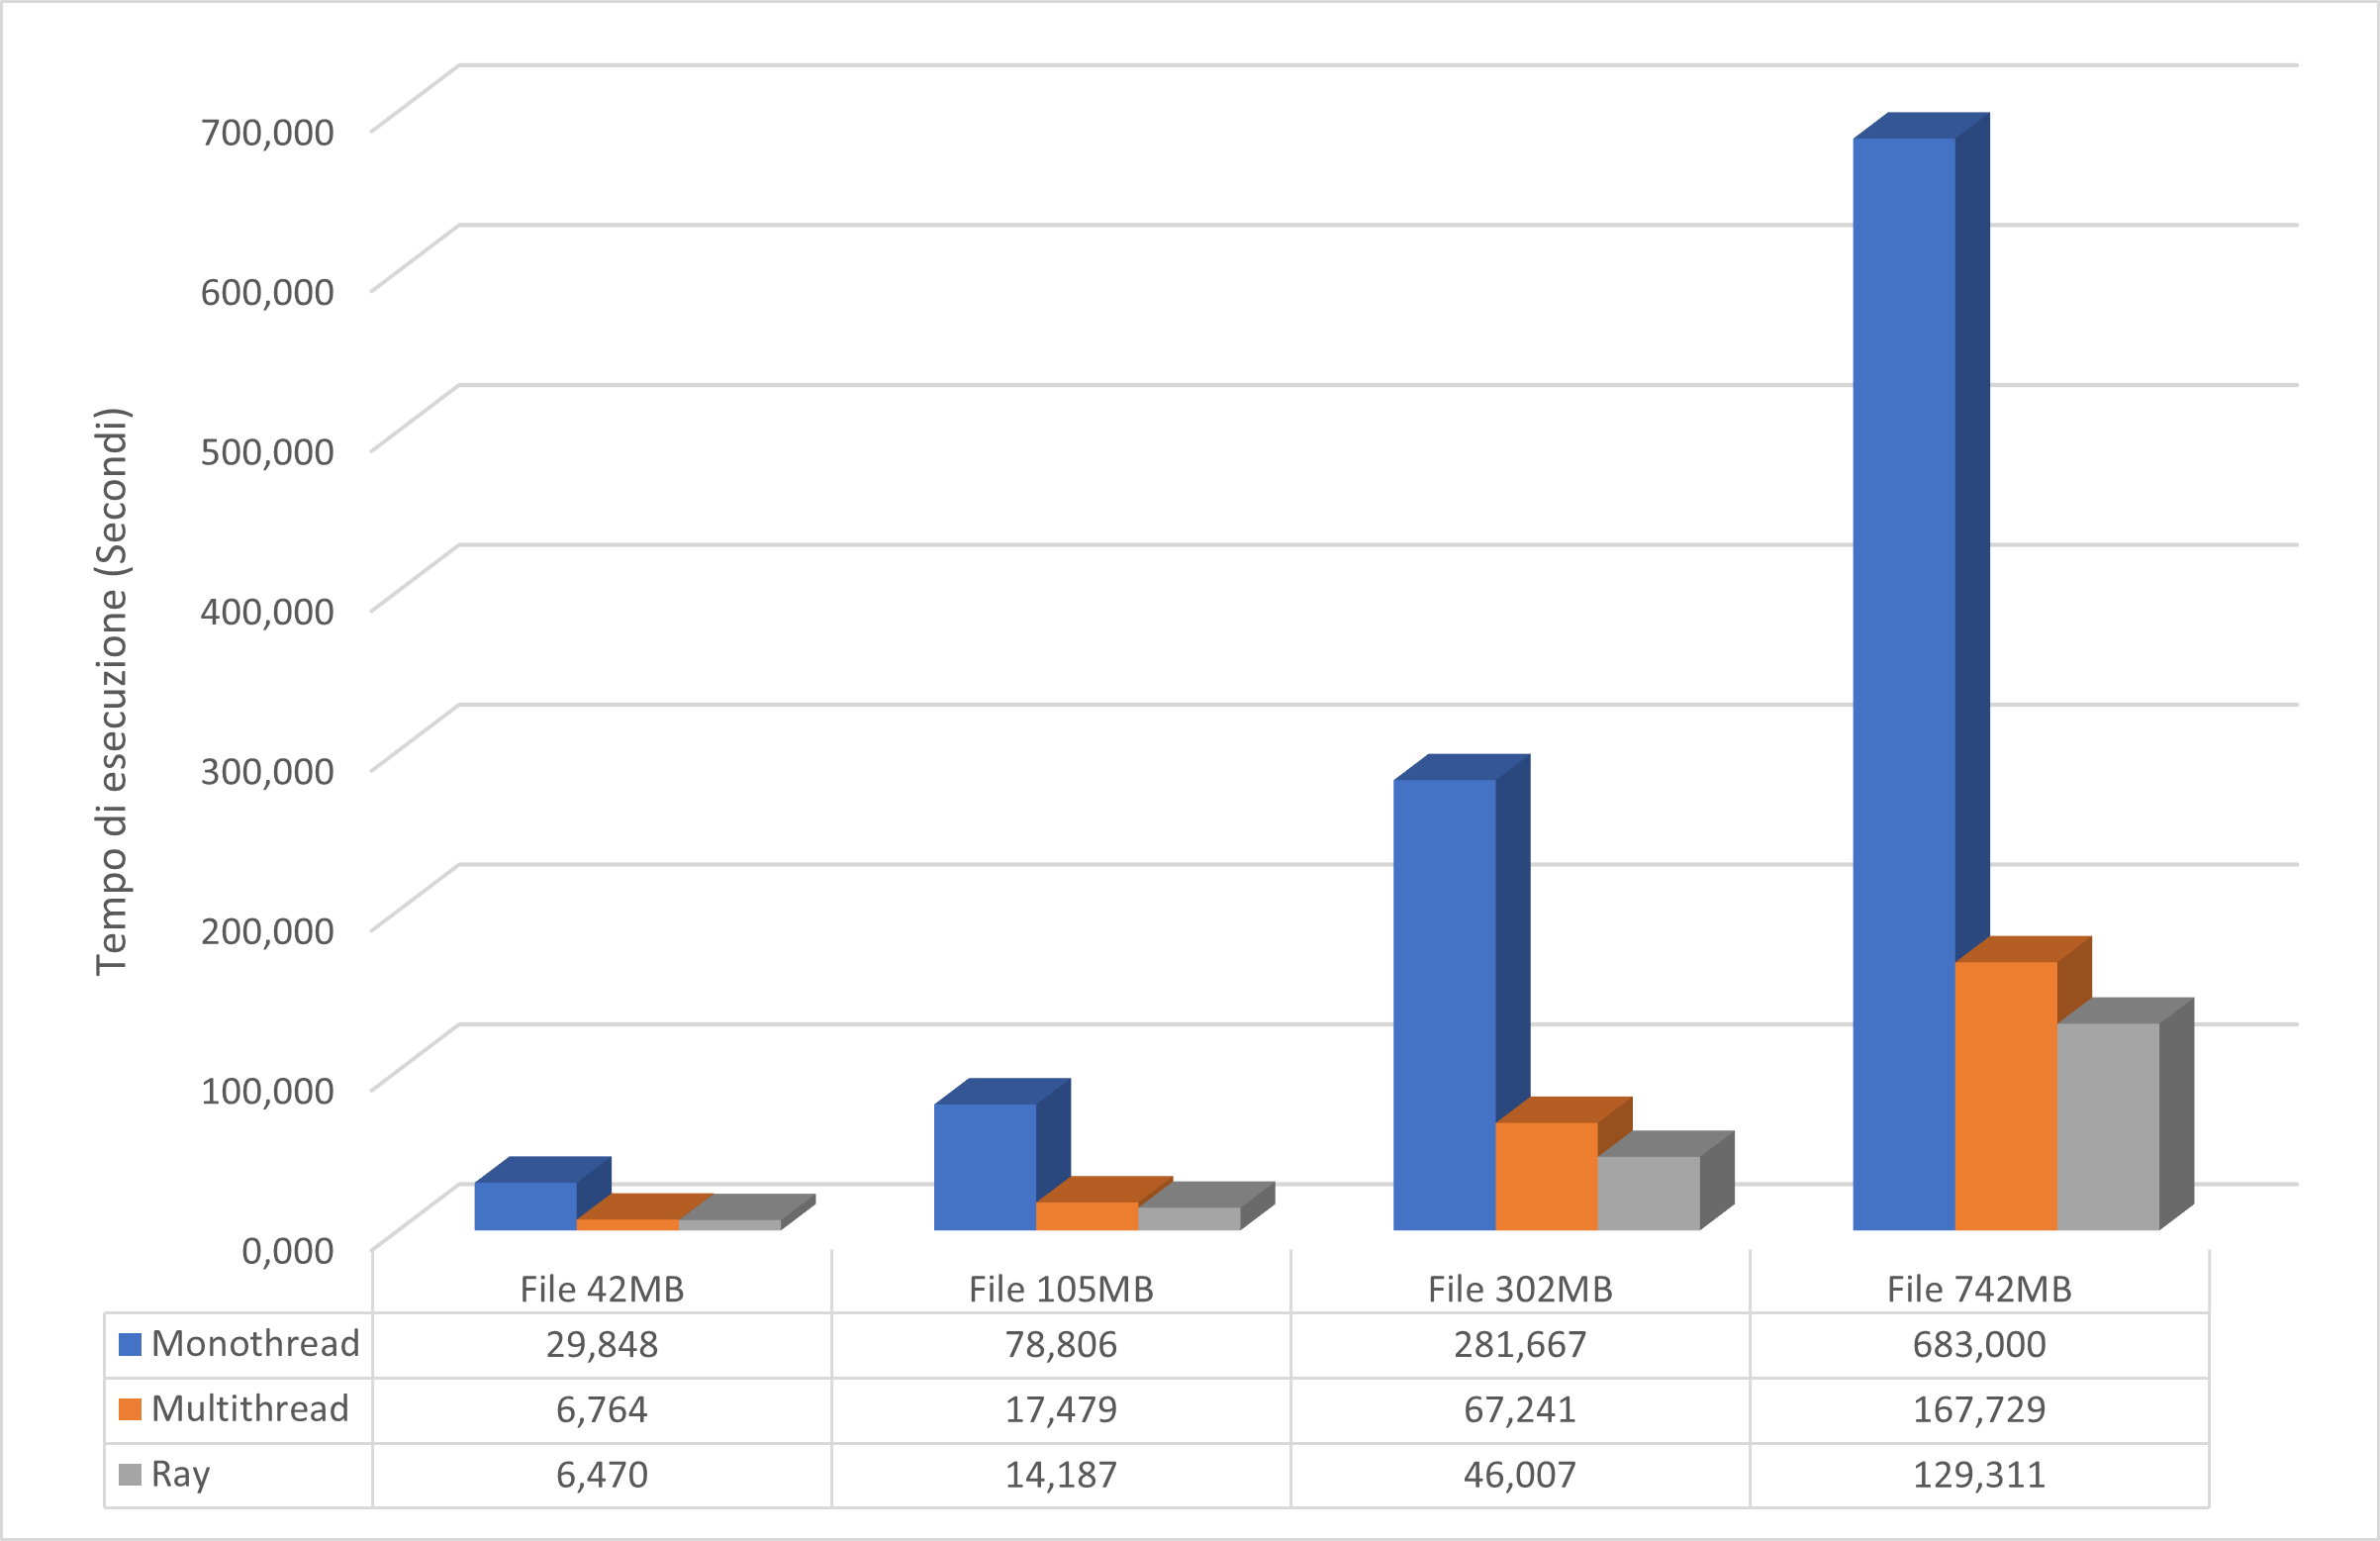
\includegraphics[width=\linewidth]{Grafico.png}
        \caption{Grafico dei tempi d'esecuzione, con tabella contenente i valori espressi in secondi}
    \end{figure}
    
    \clearpage
    
    \section{Considerazioni}
    I test sulla ricerca di sottostringhe specifiche all'interno di sequenze genomiche hanno fornito risultati significativi. Attraverso l'analisi di diverse architetture di calcolo, tra cui una versione monothread, una multithread e un'implementa-zione con Ray, è possibile osservare le differenze prestazionali delle diverse strategie di elaborazione dati in questa attività di bioinformatica.\\
    \\
    La versione monothread si è dimostrata la più lenta tra quelle analizzate, lentezza che cresce in maniera proporzionale alla grandezza del file utilizzato. Questo è dovuto al limite di utilizzo di un solo thread, che ha comportato un'esecuzione sequenziale, rendendo difficile l'analisi di sequenze genomiche di grandi dimensioni.\\
    \\
    Il multithread è emerso come un significativo passo avanti, consentendo l'elabo-razione parallela su più core. Si può osservare un notevole miglioramento delle prestazioni rispetto alla versione monothread con l'aumentare del numero di core utilizzati.\\
    \\
    Nonostante siano state riscontrate inefficienze nell'implementazione di Ray, in quanto non tutti i core a disposizione sono stati utilizzati contemporaneamente al 100\% (inefficienza che potrebbe essere attribuita a diversi fattori, tra cui la distribuzione dei dati, l'efficienza dei nodi utilizzati e la possibilità che gli stessi fossero destinati a compiti esterni al test), un ulteriore passo in avanti è stato compiuto con l'implementazione di Ray. L'uso di questa architettura ci ha permesso di sfruttare più macchine e, di conseguenza, più core contemporaneamente rispetto a quanto consentisse di fare il multithreading. L'efficienza e la scalabilità offerte da Ray sono risultate utili per affrontare grandi volumi di dati genetici.\\
    \\
    Questo progetto ha fornito informazioni sull'ottimizzazione dell'analisi delle sequenze genomiche, dimostrando come l'adozione delle giuste strategie di parallelismo possa portare a risultati notevolmente più veloci e precisi.
    
\end{document}